\documentclass[UTF8,a4paper,11pt]{ctexart}
\usepackage[margin=2.1cm,headheight=15pt]{geometry}
\usepackage{graphicx,xcolor,tabularx,booktabs,hyperref,fancyhdr,enumitem}
\usepackage{xurl}
\definecolor{ink}{HTML}{203B47}
\definecolor{accent}{HTML}{176E73}
\definecolor{soft}{HTML}{65737B}
\hypersetup{colorlinks=true,linkcolor=accent,urlcolor=accent,pdftitle={途見：基於3DGS與GMVR的澳門文旅記憶系統}}
\ctexset{section={format=\Large\bfseries\color{ink}},subsection={format=\large\bfseries\color{accent}}}
\setlength{\parindent}{2em}
\setlength{\parskip}{.4em}
\pagestyle{fancy}\fancyhf{}
\fancyhead[L]{\small\color{soft}途見｜澳門文旅記憶系統}
\fancyhead[R]{\small\color{soft}作品介紹}
\fancyfoot[C]{\thepage}
\renewcommand{\headrulewidth}{.3pt}
\begin{document}
\begin{titlepage}
\thispagestyle{empty}
\vspace*{1.1cm}
{\large\color{accent}潛能拓展創新菁英賽｜作品介紹\par}
\vspace{.6cm}
{\fontsize{32}{40}\selectfont\bfseries\color{ink}途見\par}
\vspace{.2cm}
{\LARGE\color{ink}基於 3DGS 與 GMVR 的澳門文旅記憶系統\par}
\vspace{.8cm}
{\large\color{soft}讓眼前的建築，連結可被保存、聆聽與續寫的城市記憶。\par}
\vspace{.5cm}
\begin{center}
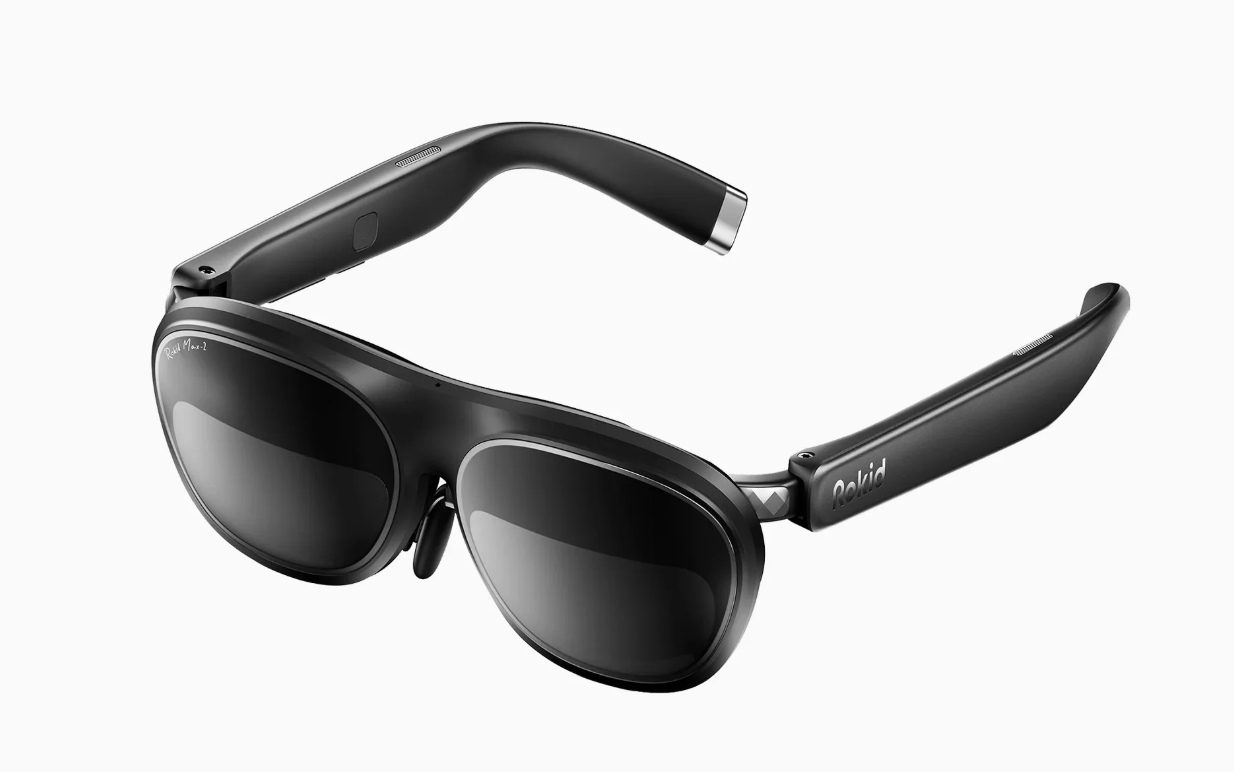
\includegraphics[width=.93\textwidth,height=8cm,keepaspectratio]{docs/assets/rokid-max2.png}
\end{center}
{\small\color{soft}圖：Rokid Max 2 產品照片。途見將其定位為現場導覽的顯示與聆聽載體；產品照片並非途見眼鏡介面實拍。\par}
\vfill
{\bfseries\color{ink}空間重建 \(\rightarrow\) 融合辨識 \(\rightarrow\) 記憶共創 \(\rightarrow\) 現場導覽與遊後回訪\par}
\vspace{.5cm}
{\small\color{soft}2026 年 10 月｜繁體中文版\par}
\end{titlepage}
\tableofcontents
\clearpage

\section{作品摘要}
「途見」是一套以澳門城市記憶為核心的文旅系統，連接 MacauSplat 重建端、網站、微信小程序與 Rokid AR 眼鏡導覽載體。作品關注大三巴等著名地標，也記錄騎樓、唐樓、街市及日常街巷中具有地方特色的普通建築。網站以三維地圖與 3DGS 實景呈現城市空間；GMVR 融合建築影像、地理位置與多視角照片，協助旅客確認眼前建築。地點編號連結真實照片、歷史資料和居民故事，使用者亦可提交文字、照片與原聲，持續補全「記憶拼圖」。小程序承接隨身查詢及行程規劃；眼鏡租借服務則讓旅客在街道現場觀看地點提示並聆聽講解。遊前選點、遊中探索與遊後回訪圍繞同一份地點資料銜接，使澳門文化記憶由一次性介紹變為可追溯、可參與、可累積的共同記錄。

\section{問題、理念與創新}
\subsection{城市記憶不只屬於著名景點}
傳統導覽容易集中於地標和固定解說。旅客走過周邊街巷時，卻未必知道眼前普通建築的名稱、來歷與居民經驗。城市文化同樣存在於老店、唐樓、街市及逐漸改變的港口與街道。若只保存少數著名建築，澳門記憶便會留下大量空白。

途見以「地點」作為共同索引：先辨認建築並確認位置，再把可查證的資料、真實照片與有同意及來源的個人敘事連起來。三維模型記錄空間面貌，照片保留某一時間的細節，人的聲音補上地圖無法表達的生活經驗。

\subsection{從單向導覽轉向共創敘事}
作品讓居民與旅客在同一地點補充不同層次的記錄。旅客可由建築認識街區，居民可講述自身經歷，教師可把地點串成探究任務，資料整理者則可核對來源、修訂錯誤。內容經過標註、同意與審核後公開，形成可持續更新的「記憶拼圖」。途見的創新不在單一硬體，而在把空間重建、建築辨識與人的記憶組成一條可延續的文化記錄流程。

\section{一套系統如何協作}
\begin{center}
\renewcommand{\arraystretch}{1.45}
\begin{tabularx}{\textwidth}{>{\bfseries\color{accent}}p{3cm}X}
\toprule
組成 & 在共同地點資料中的角色\\
\midrule
MacauSplat & 處理環繞拍攝素材，估計相機位姿並訓練 3DGS 實景模型，記錄建築的空間面貌。\\
GMVR & 結合建築區域、影像檢索、位置品質與多張照片的一致性提出地點候選，最後由使用者確認。\\
網站 & 展示三維地圖、實景模型、建築檔案及記憶內容，提供深入探索入口。\\
微信小程序 & 隨身查詢地點、收藏與安排行程，銜接遊前規劃及遊後回訪。\\
Rokid Max 2 & 租借式現場導覽載體，配合相容手機或主機顯示簡潔內容並播放講解；位置與地點資料由連接端提供。\\
\bottomrule
\end{tabularx}
\end{center}
各端以地點編號及資料目錄銜接。編號是「同一處」的身份鍵，建築照片、3DGS 場景、講解及個人記憶則是可逐步增加的內容。共用編號不等同於所有內容已即時同步；資料更新、介接頻率與版本以實際系統為準。

\section{租借眼鏡的現場導覽體驗}
在規劃的服務情境中，旅客可於指定旅遊服務點租借 Rokid Max 2，連接相容手機或配套主機後選擇語言、路線與感興趣的主題。眼鏡的目的不是取代網站或小程序，而是讓內容跟隨旅客走入真實街道：行走時提供簡潔提示，停留時顯示地點名稱並播放「小澳」的講解。

\begin{enumerate}[leftmargin=2.3em,itemsep=.45em]
\item \textbf{遊前選點：}旅客在網站或小程序選擇世界遺產、街區生活、人物事件等主題，形成可調整的探索清單。
\item \textbf{到點確認：}手機端提供定位資訊，系統查找附近景點與記憶點；相近地點或定位不佳時，旅客可透過照片辨識和人工確認避免錯配。
\item \textbf{現場觀看與聆聽：}眼鏡顯示名稱、簡短提示及步行指引，旅客聆聽「小澳」介紹；需要完整資料時，可在網站查看三維場景、歷史線索及居民故事。
\item \textbf{遊後持續回訪：}旅客可在手機端收藏地點，提交經同意的照片或故事；歸還眼鏡後，仍可用同一地點編號回看檔案。
\end{enumerate}

租借服務是途見把數碼內容帶進街道的\textbf{應用方案}。服務點設置、戶外可讀性、定位觸發、設備續航、衛生與租還流程，以及眼鏡端的實際操作方式，都須經設備和現場測試驗證。Rokid Max 2 在此是顯示與音訊載體；定位、拍攝及資料處理由相容連接端承擔，不把它們寫成眼鏡本體已完成的功能。

\section{技術方法與驗證邊界}
\subsection{三維高斯潑濺：把現場變成可重訪的空間}
MacauSplat 先以 FFmpeg 整理環繞拍攝素材，再由 COLMAP 完成影像特徵匹配、相機位姿估計及稀疏重建，最後以 Brush 訓練三維高斯潑濺（3DGS）模型，供網站展示可自由觀看的實景。模型品質取決於拍攝覆蓋、光照、位姿與訓練條件，需要按場景與版本評估。

團隊進一步利用重建所得的相機位姿與三維點雲，將建築三維包圍盒投影至多個拍攝影格，產生可供人工複核的標註資料，銜接辨識模型訓練。空間重建因此同時服務展示與資料製作。

\subsection{GMVR：用多種證據確認眼前建築}
GMVR 先以 YOLO 偵測建築區域，再以 DINOv2 特徵檢索具體建築，結合定位品質與多照片一致性排列候選，最後由使用者確認身份及位置。當建築相似或定位訊號不佳時，系統保留不確定性。這套方法的價值在於讓辨識結果能連回穩定地點、照片證據與可修訂的記憶檔案，而非聲稱在任何場景都比通用 AI 準確。

現有參考庫涵蓋\textbf{38 棟建築、335 張照片}。在\textbf{參考庫留一法}測試中，Top-1 為\textbf{88.96\%}，Top-3 為\textbf{94.93\%}。這些數值只對應該參考庫及測試條件，不能直接視為所有街景實拍的準確率。獨立實拍的融合辨識對照須與留一法分開報告，保留樣本數、拍攝條件、比較方法及錯誤案例。

\subsection{讓故事可以被查核}
建築身份、地點、歷史人物與事件線索應附資料來源；照片保留拍攝時間、來源與授權；個人故事經同意及審核後公開。未經證實的回憶以個人敘事標示，不寫成既定史實。更正及版本記錄使文化內容能持續補充，也能接受查核。

\section{文化價值與實施方向}
途見使文化傳播從「到訪著名景點」延伸至「理解街區如何生活」。旅客可以聽見建築背後的居民經驗，居民由被介紹的對象變為記憶的共同作者，學校可以把地點與線索組成實地探究任務。眼鏡降低現場接觸內容的門檻，網站承載深入觀看，小程序則讓體驗在旅途前後延續。

作品呼應澳門「1+4」經濟適度多元發展方向中做優綜合旅遊休閒業，以及「旅遊＋文化／科技」的思路，嘗試將文化關注延伸至更多社區。實際帶動效果仍應以路線使用、普通建築收錄、居民授權故事、回訪及使用者意見等資料檢驗。

面向比賽展示，可選一條真實路線貫穿全系統：拍攝及 3DGS 重建建築，以照片與定位確認地點，打開歷史資料與居民記憶，最後在眼鏡導覽情境中看提示、聽講解，並於小程序回訪。每一環節都對應可演示的介面或可複核的資料，讓作品呈現為前後相扣的系統。

\section{結語}
途見要保存的不只有澳門建築的外形，也有建築如何被辨認、被走近、被講述與被記住。三維重建給城市記憶以空間，融合辨識給它以位置，居民共創給它以聲音；可租借的 AR 眼鏡則把這些內容帶回旅客所站立的街道。從一棟樓到一條街，從一張照片到一段人生經驗，澳門的文化記憶得以被更多人看見，也由更多人共同續寫。

\section*{資料與圖片來源}
\begin{itemize}[leftmargin=2em]
\item Rokid Max 2 產品資訊：\url{https://global.rokid.com/products/rokid-max-2-ar-glasses}。封面使用參賽者指定照片，僅示意導覽載體。
\item 澳門特別行政區政府《經濟適度多元發展規劃（2024--2028 年）》：\url{https://www.gov.mo/plandiversification/zh-hant/}。
\item MacauSplat、GMVR 參考庫與測試數值依作品團隊現階段材料整理；正式提交時宜附版本、測試設定及演示記錄。
\end{itemize}
\end{document}
